\documentclass{article}
\usepackage{graphicx}
\usepackage[hidelinks]{hyperref}
\usepackage{url}

\begin{document}

\title{D-TACQ BOLO8-BLF Quickstart Guide}
\author{Sean Alsop \\ Contact: \href{mailto:sean.alsop@d-tacq.co.uk}{sean.alsop@d-tacq.co.uk} }

\maketitle

%\begin{abstract}
%The abstract text goes here.
%\end{abstract}

\tableofcontents

\section{Introduction and pre-requisites}
This document serves as a quickstart guide to the BOLO8-BLF module.
It will walk the user through the initial setup, configuration, and testing to make sure that the module is in working order.
This document relies on the user already having Control System Studio (CSS) installed on their host computer.
Installation instructions are provided on the D-TACQ ACQ400CSS GitHub repo here:
\newline
\centerline{ \href{https://github.com/D-TACQ/ACQ400CSS}{https://github.com/D-TACQ/ACQ400CSS} }
\newline
To control the unit there is a python script included in the acq400\_hapi GitHub repository.
The repo (and installation instructions) can be found here:
\newline
\centerline{ \href{https://github.com/D-TACQ/acq400_hapi}{https://github.com/D-TACQ/acq400\_hapi}. }
\newline
The script can be found in user\_apps/special/ and is named "bolo8\_cal\_cap\_loop.py".
This script is not needed for immediate use, but is needed for system calibration and shot control later in the guide.
\newpage
\subsection{Recommended reading}
\begin{enumerate}
	\item \href{http://www.d-tacq.com/resources/d-tacq-4G-acq4xx-UserGuide-r28.pdf}{The D-TACQ 4G User Guide}
	\item \href{http://www.d-tacq.com/resources/Bolo_calibration_report_user-guide.pdf}{The BOLO8-BLF User Guide}
	\item \href{https://github.com/seanalsop/bolodsp-doc/releases}{The BOLO8-BLF Software Guide}
\end{enumerate}

\section{Hardware setup and confguration}
The D-TACQ BOLO8-BLF test panel uses a ZIF (zero insertion force) socket to hold the bolometer and allows the user to measure various test points on the bolometer when in use.
This is the panel D-TACQ recommend using initially.
Once the bolometer has been fitted to the test panel the user can connect the panel to the front of the BOLO8-BLF module.
Figure \ref{boloZIFimage} shows a bolometer sitting in the test panel ZIF socket.
Figure \ref{boloZIFconnctedImage} shows the same test board connected to the BOLO8-BLF mezzanine in the acq2106 carrier.

\begin{figure}
    \centering
    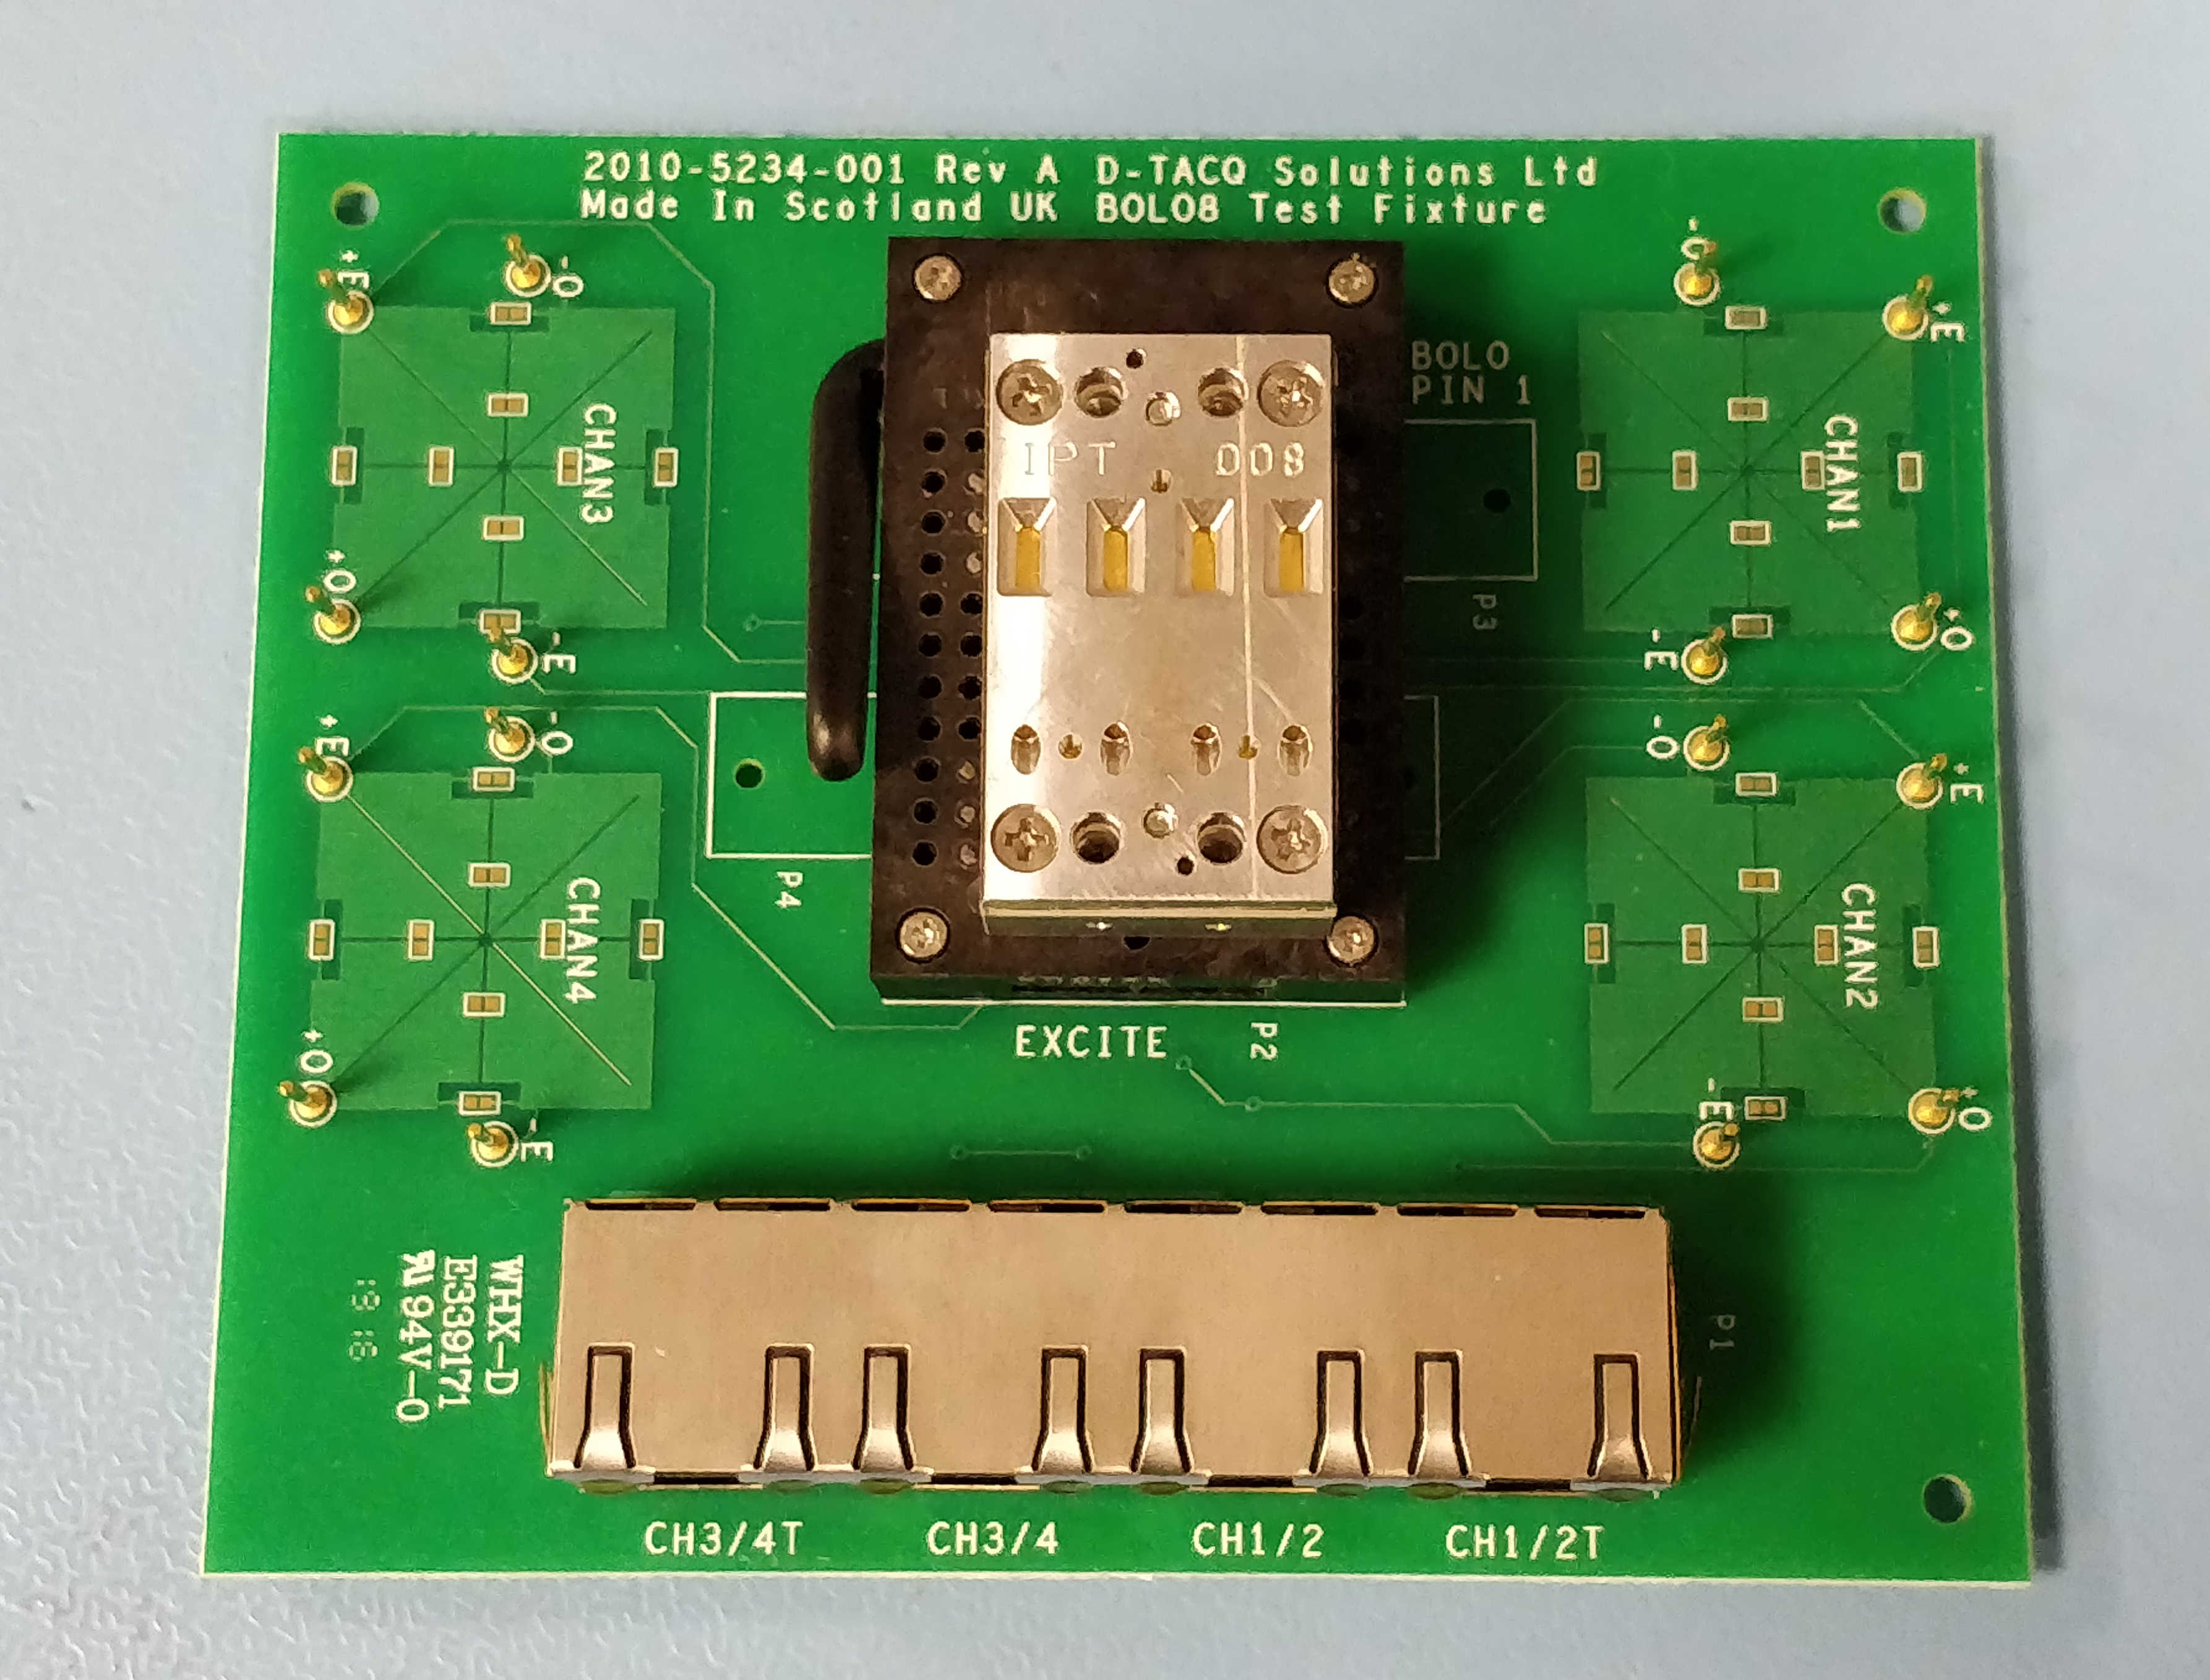
\includegraphics[width=5.0in]{images/bolo-zif.jpg}
    \caption{A bolometer sitting in the test board ZIF socket}
    \label{boloZIFimage}
\end{figure}

\begin{figure}
	\centering
	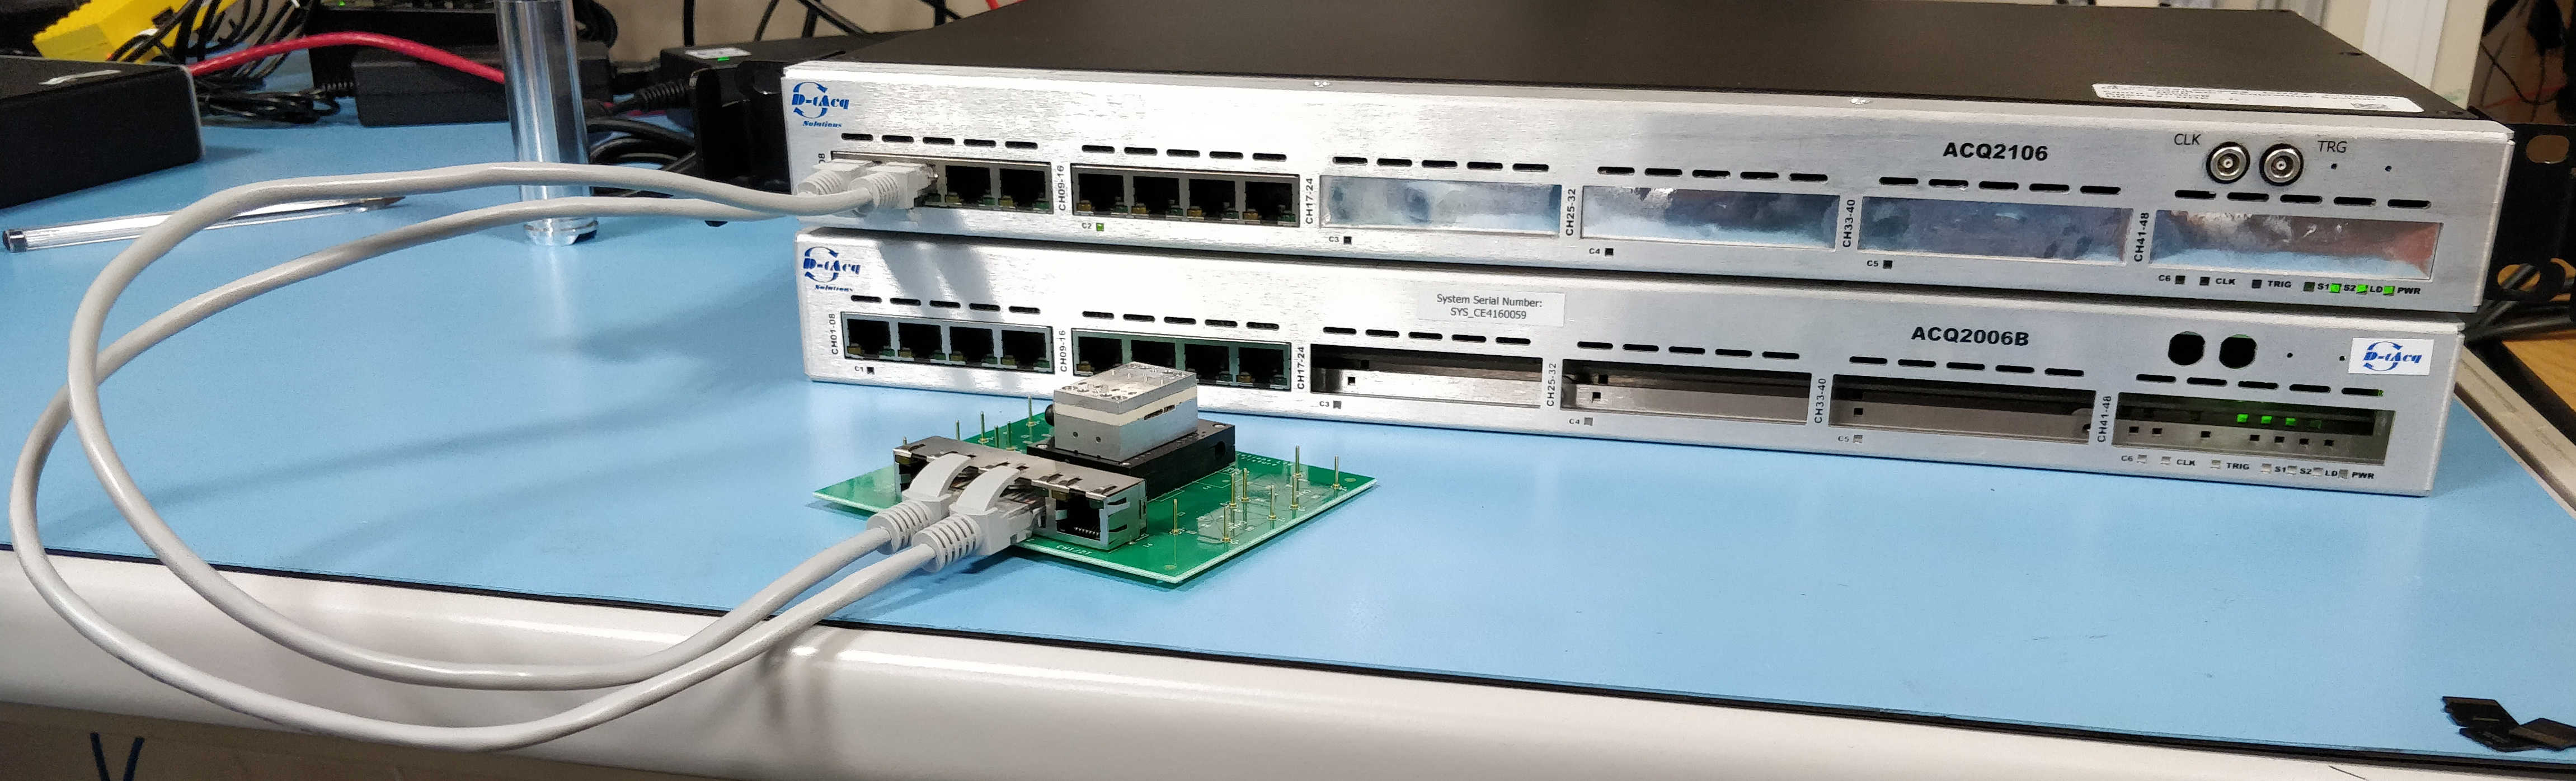
\includegraphics[width=5.0in]{images/bolo-zif-connected.jpg}
	\caption{A bolometer sitting in the test board ZIF socket connected to an acq2106 system.}
	\label{boloZIFconnctedImage}
\end{figure}

\newpage

\section{Using CS Studio to stream live data}
CS Studio can be used to stream lower rate data from the acq2106.
This is extremely useful for initial validation and testing as it allows the user to verify that the system is working very quickly.
Once CS Studio has been installed according to the instructions contained in the GitHub repo the BOLO8 Launcher can be opened from the project window.
There are several channels on the BOLO8-BLF module, but the voltage magnitude (MAG) works well for this test.
Click on the MAG button in the "Live Plot" container, and also open the Capture OPI.
To see the shark-fin shown in figure \ref{bolocss3finnocal} there was a bicycle light placed on top of the bolometer.
The shark-fin shape is the data acquired as the foils heat up and cool down as the continuously flashing bicycle lamp turns on and off.
Note that the channels have not yet been calibrated and so the offsets have not been accounted for yet.
This means that some channels likely will be visually offset from one another.
In figure \ref{bolocss3finnocal} this can be observed on the first three channels.

\begin{figure}
	\centering
	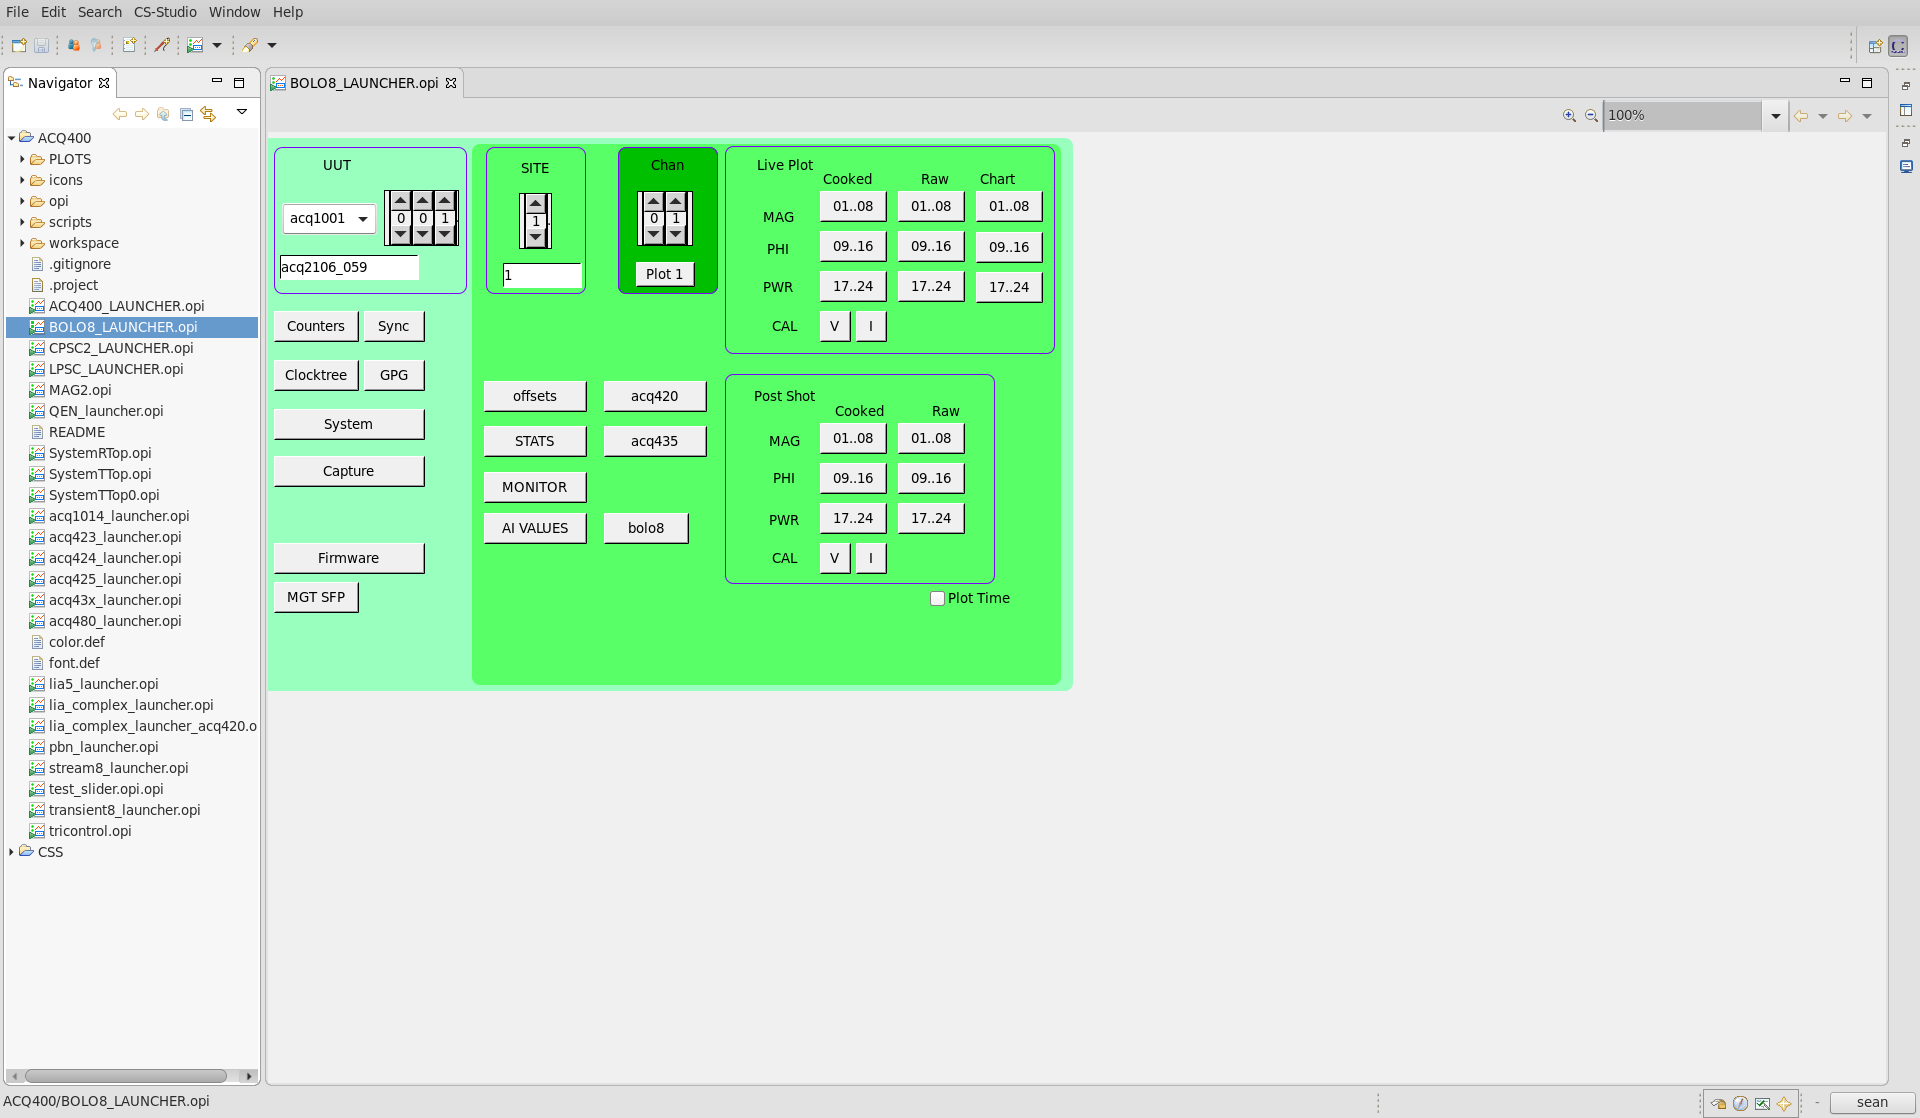
\includegraphics[width=5.0in]{images/css_launcher.png}
	\caption{A CS Studio screen showing where to access the correct BOLO8 launcher.}
	\label{bolocsslauncher}
\end{figure}

\begin{figure}
	\centering
	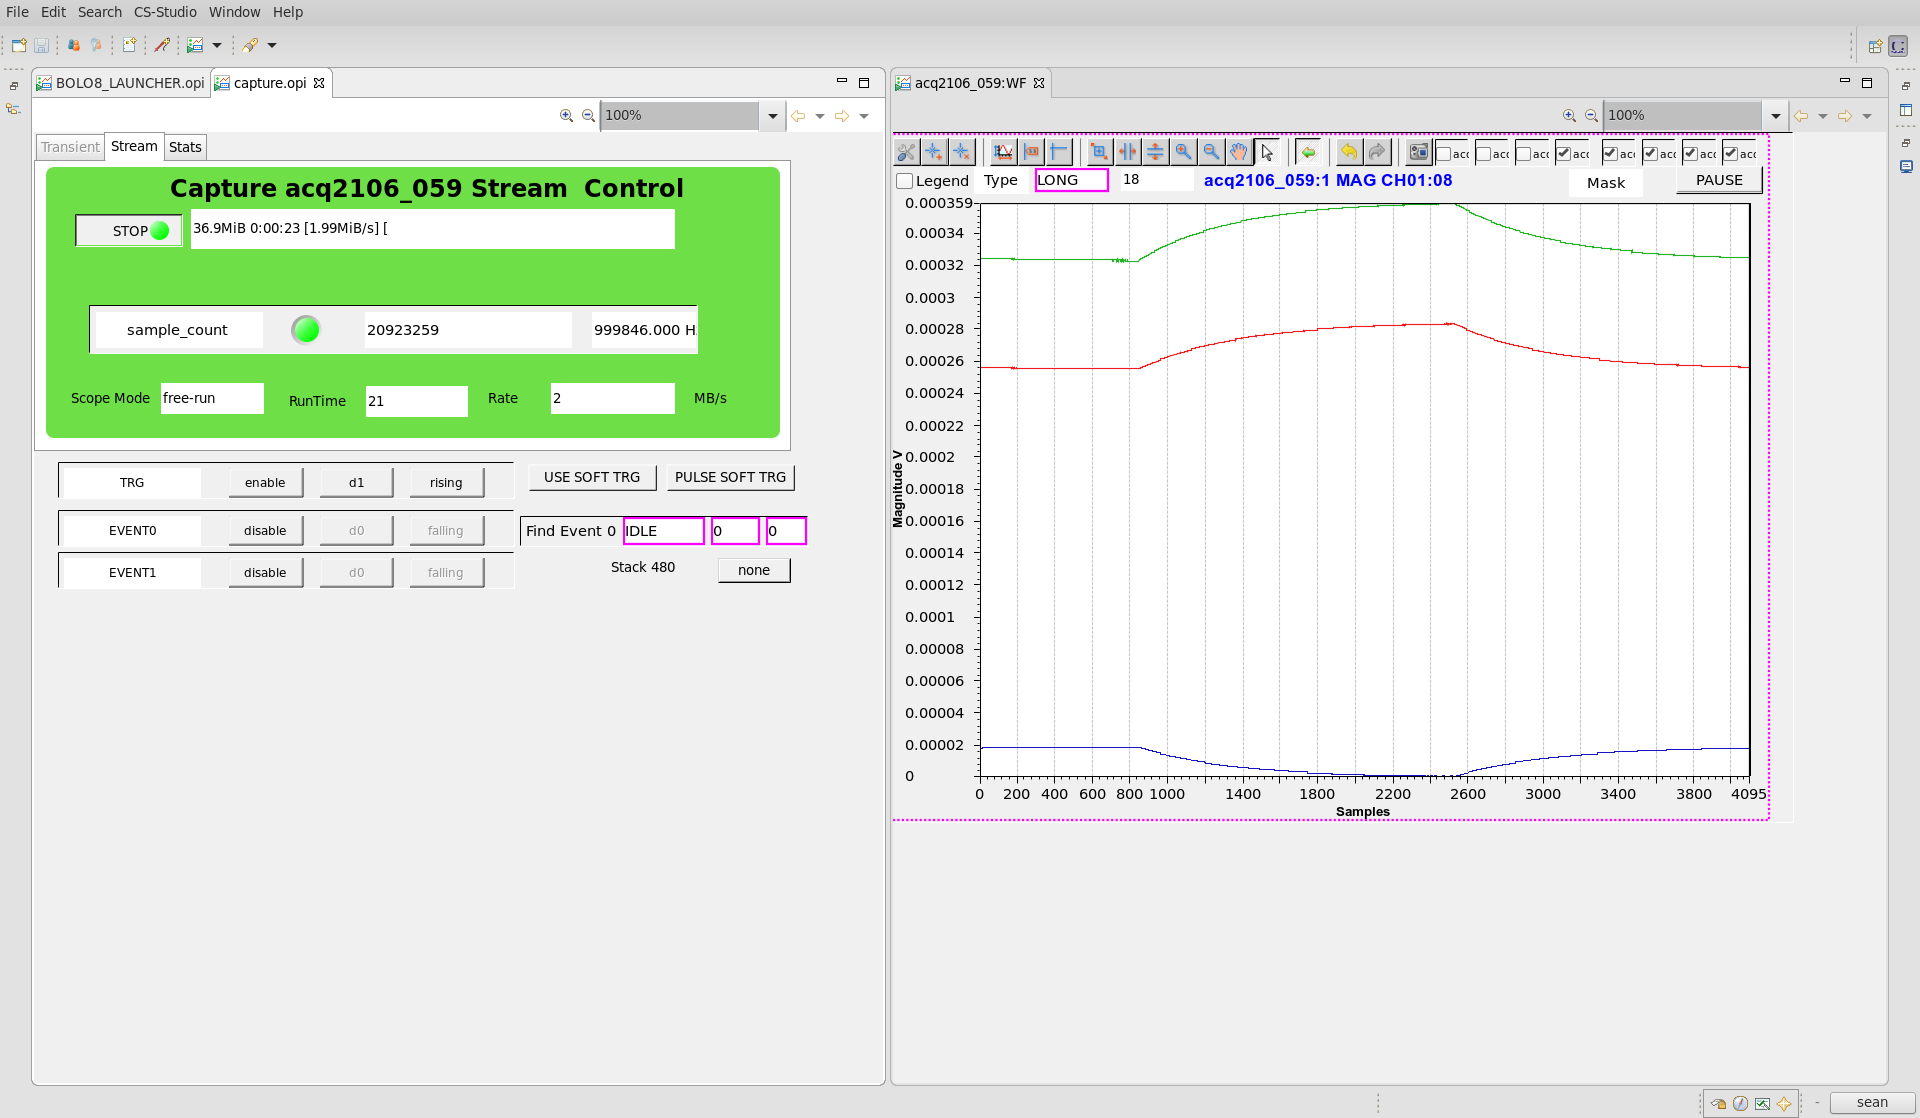
\includegraphics[width=5.0in]{images/3-fin-no-cal.png}
	\caption{A CS Studio screen showing 3 channels without calibration. Note the offsets between channels.}
	\label{bolocss3finnocal}
\end{figure}

\begin{figure}
	\centering
	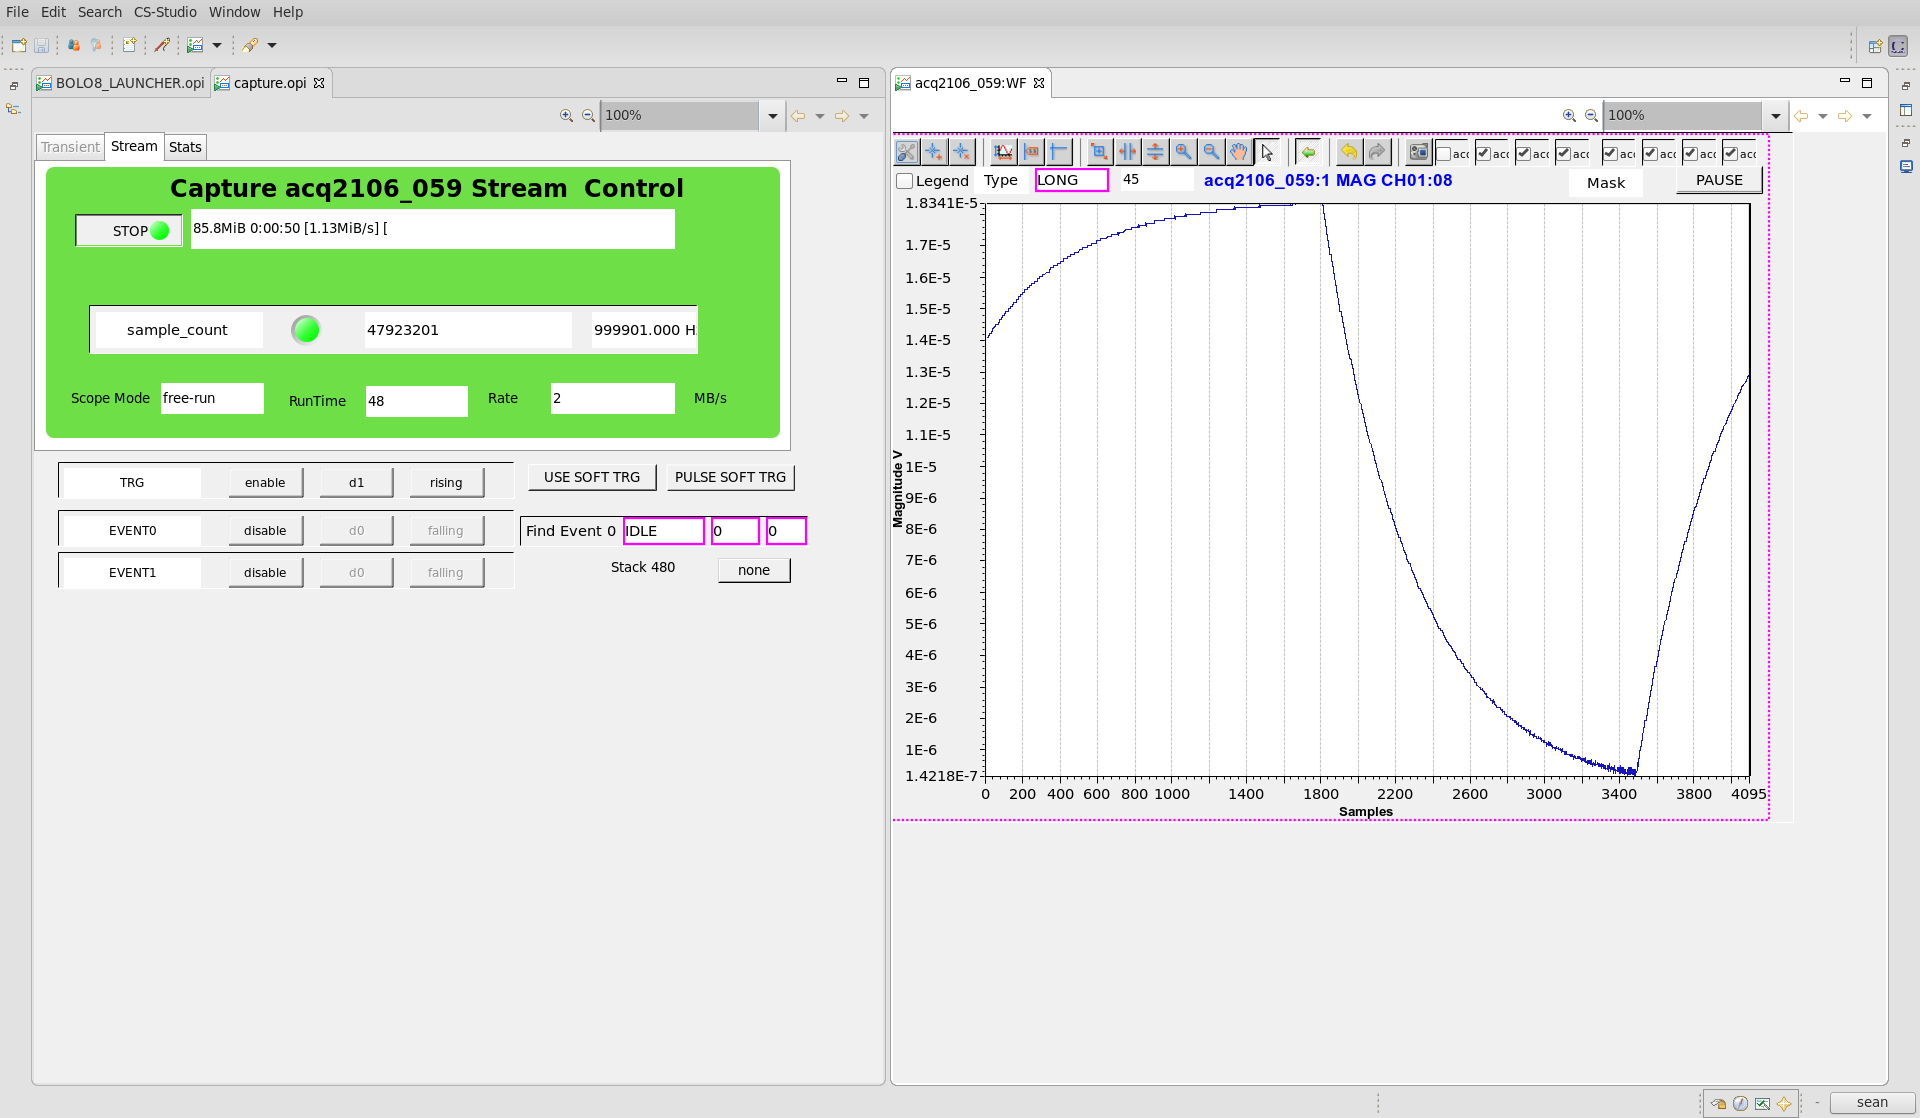
\includegraphics[width=5.0in]{images/1-fin-no-cal.png}
	\caption{The capture and MAG stream OPIs open with a sharkfin on the MAG OPI.}
	\label{bolocsscapture}
\end{figure}

\newpage

\section{Using python to calibrate the system}
To calibrate the system it is recommended that the bolo8\_cal\_cap\_loop.py python script is used.
This can be found in the HAPI python library provided by D-TACQ mentioned previously in this document.
Remember to remove the flashing bicycle lamp from the vicinity of the bolometer when calibrating the BOLO8-BLF module.
\newline
To calibrate the acq2106 first connect to the acq2106 using ssh and edit the following file:

\begin{verbatim} /mnt/local/sysconfig/bolo.sh \end{verbatim}

and select which channels you wish to calibrate by changing the following line.

\begin{verbatim} BOLO_ACTIVE_CHAN="1 2 3 4" \end{verbatim}

Once the desired calibration channels have been chosen the python script can than be run from the host computer like so:

\begin{verbatim} python bolo8_cal_cap_loop.py --cal=1 --cap=0 --shots=1 acq2106_123\end{verbatim}

\newpage

\section{Performing the same test after a calibration}
The same CS Studio test can be performed after having calibrated the system.
Figure \ref{3fincal} only shows 3 fins because the bolometer at use for testing at D-TACQ only has 3 working foils.
Note that all of the channels are now offset from the same value (very close to 0 volts).
The fins having varying heights can be attributed to the torch being positioned at an angle above the bolometer and the light from it being distributed unevenly.

\begin{figure}
	\centering
	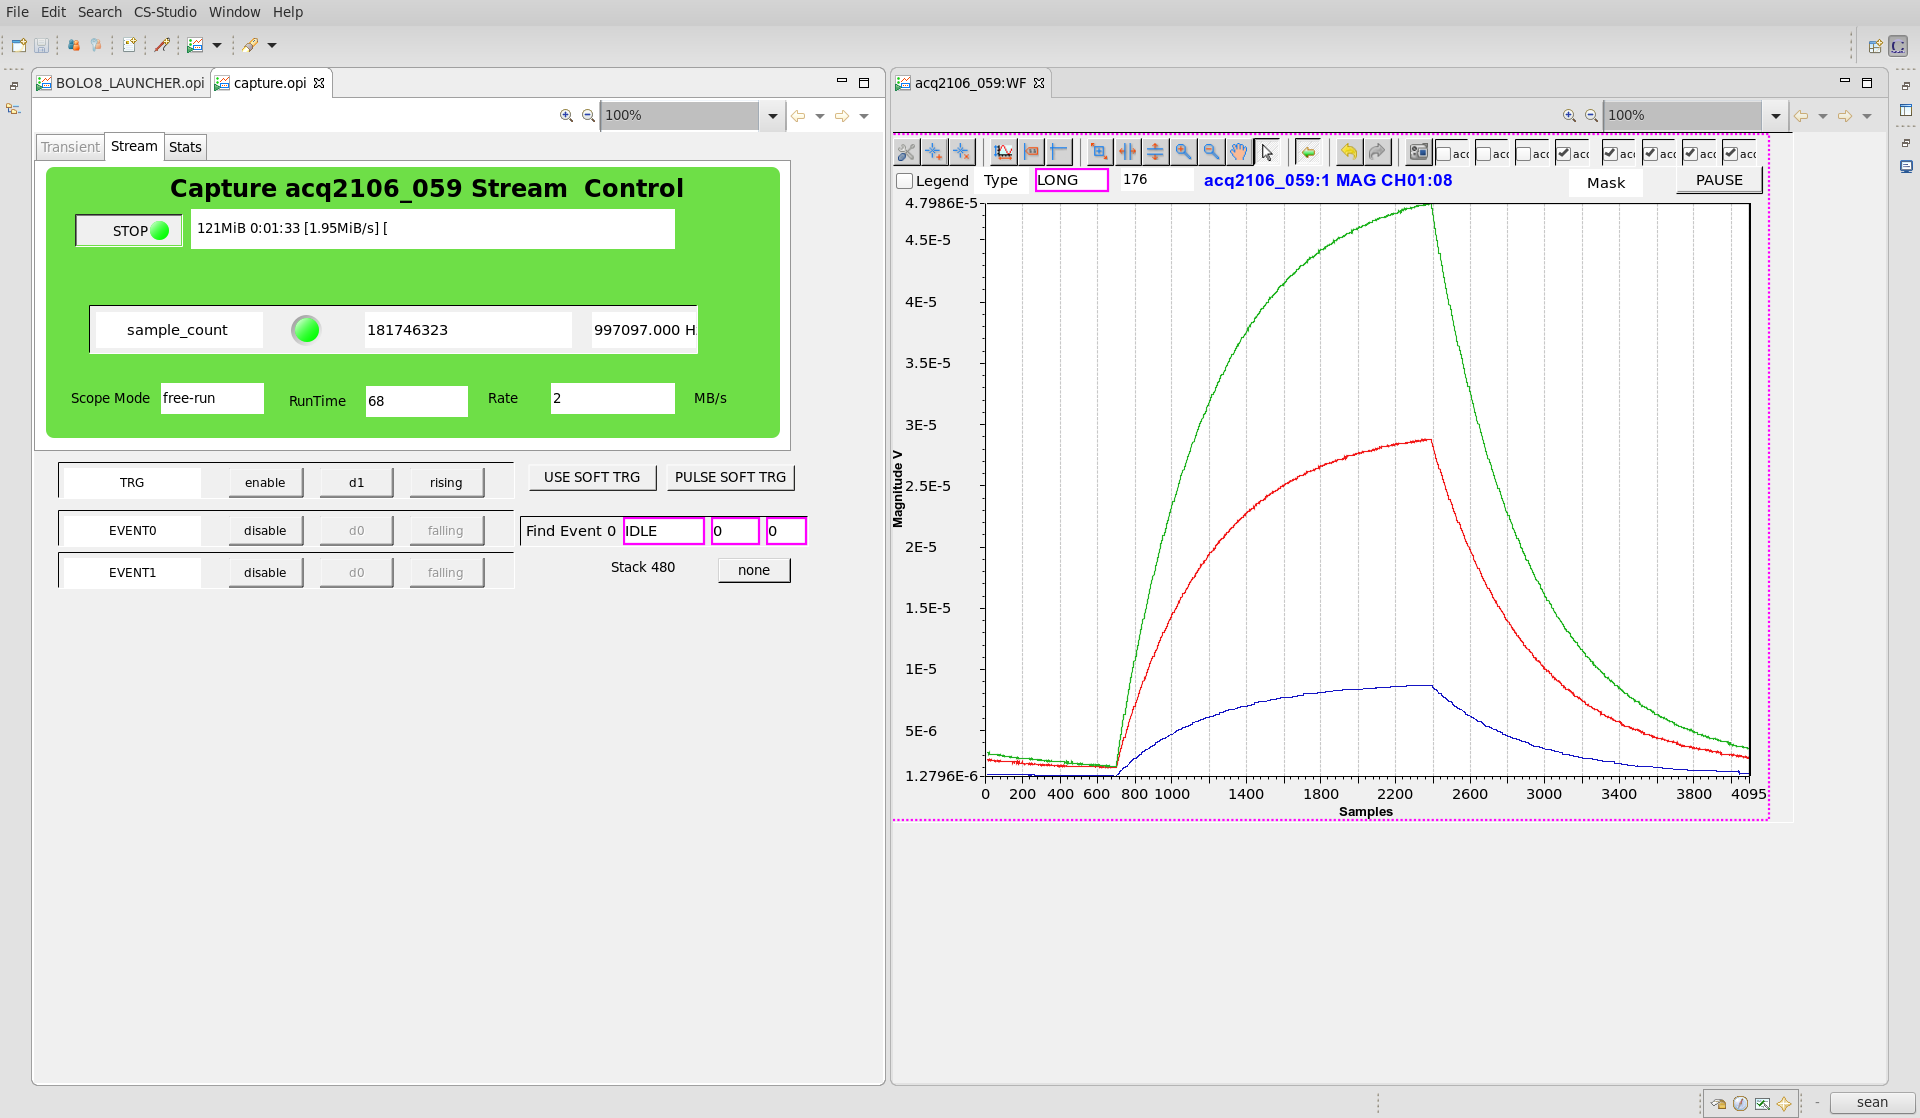
\includegraphics[width=5.0in]{images/3-fin-cal.png}
	\caption{A CS Studio screen showing 3 channels after a calibration has been performed. Note the offsets have disappeared.}
	\label{3fincal}
\end{figure}


\section{Conclusion}
This document has illustrated the recommended method for testing a D-TACQ acq2106 fitted with the BOLO8-BLF mezzanine.
The recommended steps are to insert the bolometer in the D-TACQ bolomter test panel ZIF socket and connect the panel to the acq2106.
Once CS Studio is installed the user can stream data from the acq2106 and use a flashing bicycle lamp to inspect the shark fin shape in the resultant data. Calibration removes the offsets observed in a non-calibrated system. 

\end{document}